Fourier’s Law of Heat conduction is given by the following equation:
\begin{equation}\label{eq:HeatFlux}
    Q^{'} = -kA\frac{dT}{dx}
\end{equation}
where
$Q^{'}$ = Heat flux (rate of heat transfer)

\begin{figure}[h!]
    \begin{center}
        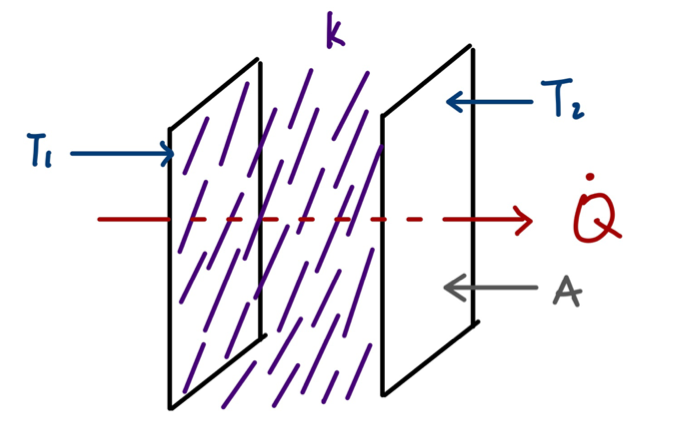
\includegraphics[width=0.45\textwidth]{Fourier.png}
    \end{center}
    \caption{Fourier's equation}
\end{figure}

$k$ = The thermal conductivity of the material to which heat is being transferred 

$A$ = Cross-sectional area of surface that heat is being transferred to

Fourier’s Law assumes that the system is in steady state -- i.e. the temperature of the source of heat stays constant \cite{DaianJeanFrancois2014}. Heat flux ($Q^{'}$) is the rate at which heat energy is transferred between two points in the system. We can analyse that the heat flux is proportional to temperature gradient.

According to the equation, we designed 6 experiments to find out the variation of heat flux by finding the thermal gradient of each experiments. At high temperature, yeast will denature and become chemically inactive, and at low temperatures, fermentation will be inefficient. Neither will give a good yield production. Thus, the temperature of heating plate needs to be considered to maintain the temperature within the range. We aimed to design an insulation system that minimises heat loss to the surroundings while heating temperature range being kept within 28-33\si{\celsius} \cite{LIU20191}.  